\documentclass[border=1cm]{standalone}
\usepackage{tikz}

% Define recursive function for Sierpiński carpet
\makeatletter
\newcommand\SierpinskiCarpet[4]{% x, y, size, depth
    \pgfmathparse{#4 == 0}%
    \ifnum\pgfmathresult=1\relax%
        % Draw a filled square
        \fill[black] (#1,#2) rectangle (#1+#3,#2+#3);%
    \else%
        % Calculate new size (1/3 of original)
        \pgfmathsetmacro{\newsize}{#3/3}%
        % Draw the 8 smaller carpets (excluding center)
        \SierpinskiCarpet{#1}{#2}{\newsize}{\numexpr#4-1\relax}% bottom-left
        \SierpinskiCarpet{#1+\newsize}{#2}{\newsize}{\numexpr#4-1\relax}% bottom-middle
        \SierpinskiCarpet{#1+2*\newsize}{#2}{\newsize}{\numexpr#4-1\relax}% bottom-right
        
        \SierpinskiCarpet{#1}{#2+\newsize}{\newsize}{\numexpr#4-1\relax}% middle-left
        % Skip center square (this creates the "hole")
        \SierpinskiCarpet{#1+2*\newsize}{#2+\newsize}{\newsize}{\numexpr#4-1\relax}% middle-right
        
        \SierpinskiCarpet{#1}{#2+2*\newsize}{\newsize}{\numexpr#4-1\relax}% top-left
        \SierpinskiCarpet{#1+\newsize}{#2+2*\newsize}{\newsize}{\numexpr#4-1\relax}% top-middle
        \SierpinskiCarpet{#1+2*\newsize}{#2+2*\newsize}{\newsize}{\numexpr#4-1\relax}% top-right
    \fi%
}
\makeatother

\begin{document}
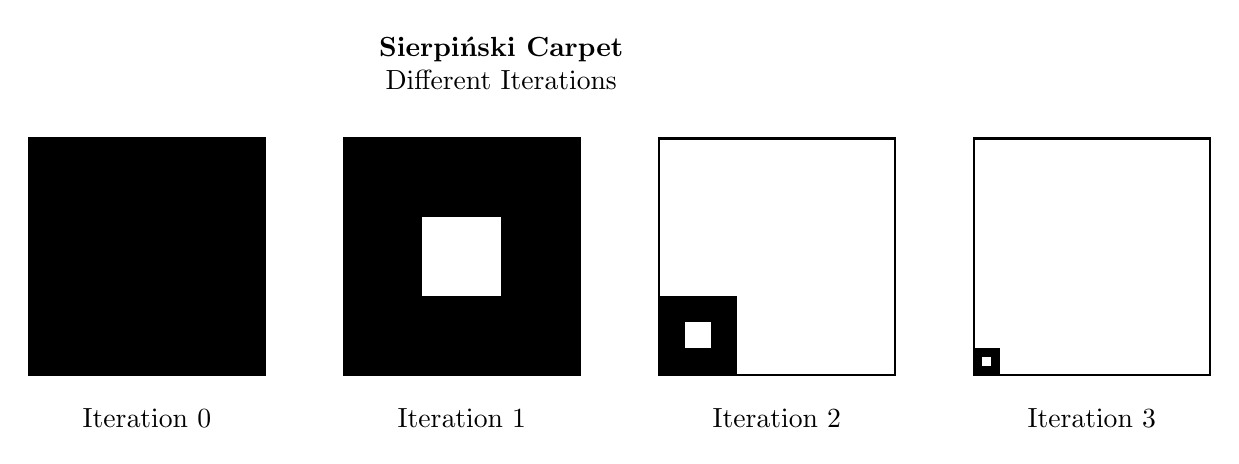
\begin{tikzpicture}
    % Generate Sierpiński carpets for different iterations
    \foreach \iteration in {0,1,2,3} {
        \begin{scope}[xshift=\iteration*4cm]
            % Draw the border
            \draw[black, thick] (0,0) rectangle (3,3);
            % Generate Sierpiński carpet
            \SierpinskiCarpet{0}{0}{3}{\iteration}
            % Add iteration label
            \node[below] at (1.5,-0.3) {Iteration \iteration};
        \end{scope}
    }
    
    % Add title
    \node[align=center, above] at (6,3.5) {\textbf{Sierpiński Carpet}\\Different Iterations};
\end{tikzpicture}
\end{document}